
\newlength{\originalVOffset}
\newlength{\originalHOffset}
\setlength{\originalVOffset}{\voffset}
\setlength{\originalHOffset}{\hoffset}

\setlength{\voffset}{0cm}
\setlength{\hoffset}{0cm}

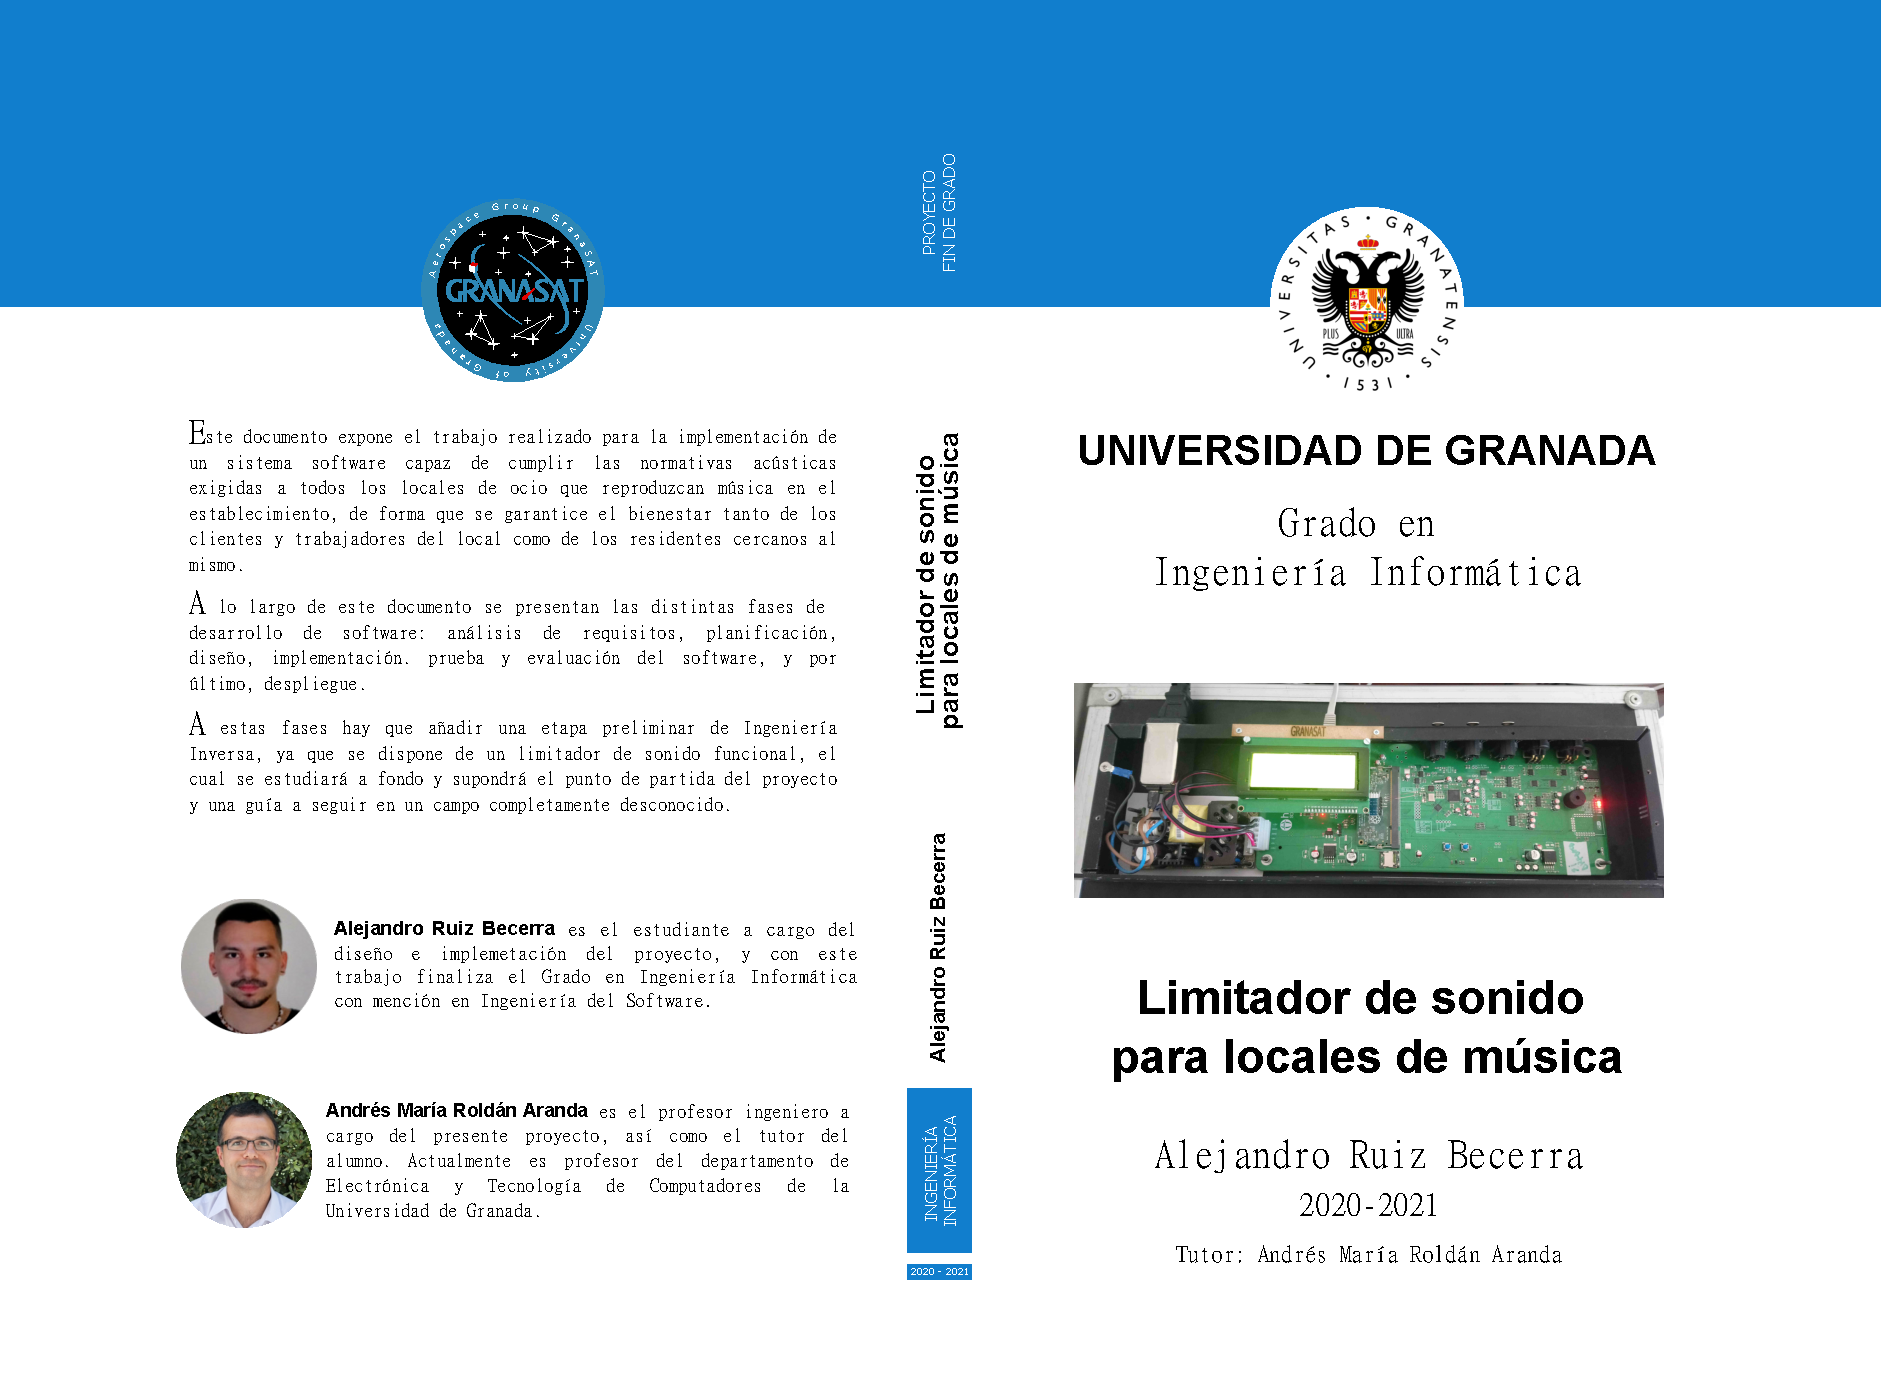
\includepdf[pages=-,link=true,landscape]
{./portada/portada_tfg.pdf}

\setlength{\voffset}{\originalVOffset}
\setlength{\hoffset}{\originalHOffset}

\addcontentsline*{toc}{chapter}{\numberline{}{}}

\pagenumbering{roman} \setcounter{page}{1}
\thispagestyle{empty}
\vspace*{3cm}
\newpage


\begin{center}
\textbf{\huge 
\includegraphics[scale=1.45]{figuras/logo_ugr.pdf}}
\par\end{center}{\huge \par}

\begin{center}
\vspace*{1cm}
\par\end{center}

\begin{center}
\textbf{\large GRADO EN}\\
\textbf{\large INGENIERÍA INFORMÁTICA}
\par\end{center}{\large \par}

\begin{center}
{\large TRABAJO DE FIN DE GRADO}

\par\end{center}{\large \par}

\begin{center}
\par\end{center}

\begin{center}
\textbf{\emph{\LARGE {Limitador de sonido}}} \\
\textbf{\emph{\LARGE {para locales de música}}}
\par\end{center}{\LARGE \par}

\begin{center}
\vspace*{3cm}
\par\end{center}

\begin{center}
{\large CURSO ACADÉMICO: 2020 - 2021}
\par\end{center}{\large \par}

\begin{center}
{\large Alejandro Ruiz Becerra}
\par\end{center}{\large \par}

\newpage
\thispagestyle{empty}

~

\newpage
\thispagestyle{empty}

\begin{center}

\includegraphics[scale=1.45]{figuras/logo_ugr.pdf}
\par\end{center}

\begin{center}
GRADO EN INGENIERÍA INFORMÁTICA\par\end{center}

\begin{center}
\vspace*{0.1cm}
\par\end{center}

\begin{center}
\textbf{\emph{\LARGE {Limitador de sonido}}} \\
\textbf{\emph{\LARGE {para locales de música}}}
\par\end{center}{\Large \par}

\begin{center}
\vspace*{0.3cm}
\par\end{center}

\begin{center}
REALIZADO POR:
\par\end{center}

\begin{center}
\textbf{Alejandro Ruiz Becerra}
\par\end{center}

\begin{center}
DIRIGIDO POR:
\par\end{center}

\begin{center}
\textbf{Andrés María Roldán Aranda}
\par\end{center}

\begin{center}
DEPARTAMENTO:
\par\end{center}

\begin{center}
\textbf{Electrónica y Tecnología de Computadores}
\par\end{center}

\begin{center}
\vfill
\par\end{center}

\vspace*{1.5cm}

\newpage
\thispagestyle{empty}
\noindent
\blankpage

%Begin ----  Para que funcione bien el TOC en PDF
\clearpage
\thispagestyle{empty}
\phantomsection
\addcontentsline{toc}{chapter}{Autorización Lectura}

\noindent D. Andrés María Roldán Aranda, Profesor del Departamento
de Electrónica y Tecnología de los Computadores de la Universidad
de Granada, como director del Trabajo Fin de Grado de D. Alejandro Ruiz Becerra,

\vspace*{1cm}

Informa:

\begin{doublespace}
Que el presente trabajo, titulado:
\end{doublespace}

\begin{doublespace}
\begin{center}
\textbf{\emph{\large {}Limitador de sonido para locales de música}}
\par\end{center}{\large \par}
\end{doublespace}

\noindent ha sido realizado y redactado por el mencionado alumno bajo
mi dirección, y con esta fecha autorizo a su presentación.

\vspace*{1cm}

\begin{center}
Granada, a 2 de septiembre de 2021
\par\end{center}

\bigskip
\bigskip
\begin{center}

\includegraphics[scale=0.2]{imagenes/firmaTutor.png}
\end{center}

\begin{center}
\begin{doublespace}
Fdo. Andrés María Roldán Aranda
\end{doublespace}
\end{center}

\newpage
\thispagestyle{empty}
\noindent

\newpage
\phantomsection
\noindent
\blankpage

\addcontentsline{toc}{chapter}{Autorización Depósito Biblioteca}
\bigskip

\noindent Los abajo firmantes autorizan a que la presente copia de
Trabajo Fin de Grado se ubique en la Biblioteca del Centro y/o
departamento para ser libremente consultada por las personas que lo
deseen.

\vspace*{1cm}

\begin{center}
Granada, a 2 de septiembre de 2021
\par\end{center}

\bigskip
\bigskip

\begin{center}
\hspace{0cm}

\includegraphics[width=0.35\textwidth]{imagenes/firmaAlumno.jpg}
\hspace{3cm}

\includegraphics[width=0.35\textwidth]{imagenes/firmaTutor.png}
\end{center}

\begin{doublespace}
\begin{center}
\hspace{0cm}Fdo. Alejandro Ruiz Becerra \hspace{3cm} Fdo. Andrés María Roldán Aranda
\end{center}
\end{doublespace}
~

%Begin ----  Para que funcione bien el TOC en PDF
\clearpage
\phantomsection
\noindent
\thispagestyle{empty}


\addcontentsline{toc}{chapter}{Resumen}
\vspace{-1.48cm}
\begin{center}
%\begin{adjustwidth}{-9pt}{0pt}
    \textbf{\Large Limitador de sonido para locales de música}
%\end{adjustwidth}
\par\end{center}{\Large \par}

\begin{center}
    \textbf{\large Alejandro Ruiz Becerra}
    \par\end{center}{\large \par}

\vspace{0.75cm}


\begin{doublespace}
    \noindent \textbf{PALABRAS CLAVE:}
\end{doublespace}


\begin{singlespace}
    \noindent GranaSAT, Acústica y audio, Ingeniería Acústica, Ingeniería Inversa, Control de ruidos, Ecualización, Electrónica.
\end{singlespace}

\begin{doublespace}
    \noindent \textbf{RESUMEN:}
\end{doublespace}

\begin{singlespace}
    \noindent El objetivo del presente proyecto es diseñar e implementar el software necesario para la construcción de un limitador de sonido para locales de ocio, de forma que se cumplan las especificaciones legales y ordenanzas exigidas por las instituciones en éste ámbito, siendo beneficiara del presente trabajo la empresa \textbf{Heimdal Sound Control}.

    \noindent El proyecto puede dividirse en tres grandes bloques: ingeniería inversa, diseño e implementación. Durante la primera fase se estudian y analizan limitadores de sonido de la competencia, ya presentes en el mercado; para luego diseñar el sistema en base a los requisitos extraídos del proceso de ingeniería inversa, y finalmente desarrollar y probar el software del producto.

    \noindent Este Trabajo de Fin de Grado se sitúa en el ámbito de un proyecto mayor, ambicioso y de largo recorrido, y se apoya en el trabajo realizado por otros alumnos pertenecientes a diversas competencias. Por tanto, el presente trabajo no debe verse como un todo, sino como un gran engranaje dentro de una máquina mayor, el cuál permite que el conjunto de componentes interaccionen entre ellos.

    \noindent La complejidad y el ámbito multidisciplinar de este Trabajo de Fin de Grado permite cubrir, no sólo algunas de las diferentes especialidades del Grado en Ingeniería Informática, sino también adquirir conocimientos y habilidades transversales o específicos de otros campos de la Ingeniería, como la \textbf{Electrónica} y la \textbf{Acústica}.

    \noindent El resultado de todo lo expuesto culmina con un equipo real de limitación de sonido completo y funcional, que cumple con los requisitos definidos en las etapas iniciales del proyecto, y con el cual se cierra la etapa universitaria de Grado.
\end{singlespace}

\vspace{1.25cm}
\newpage
\vspace{-1.15cm}

\begin{otherlanguage}{english}

\begin{center}
\textbf{\Large Sound limiter for music venues}
\par\end{center}{\Large \par}

\begin{center}
\textbf{\large Alejandro Ruiz Becerra}
\par\end{center}{\large \par}

\vspace{0.75cm}
\begin{doublespace}
\noindent \textbf{KEYWORDS:}
\end{doublespace}

\begin{singlespace}

    \noindent GranaSAT, Acoustics and audio, Acoustical Engineering, Reverse Engineering, Noise control, Equalization, Electronics.

\end{singlespace}

\begin{doublespace}
\noindent \textbf{ABSTRACT:}
\end{doublespace}

\begin{singlespace}

    \noindent The main objective of this project is to design and implement the required software to build a sound limiter for music venues, so that the legal specifications and ordinances demanded by the institutions are enforced, being benefited of the current work the \textbf{Heimdal Sound Control} company.

    \noindent The project can be divided in three blocks: reverse engineering, design and implementation. During the first phase, a functional sound limiter out of the market will be analyzed and investigated. As a result, our system's design will be based on the functional and non-functional requirements out of the reverse engineering process. Finally, the system's software will be implemented and tested accordingly.

    \noindent This Bachelor's Thesis is under the scope of a bigger, ambitious and long-run project; and is based on the work of other students from different competences. Therefore, the current work should not be seen as a whole, but as a big gear inside a bigger machine, which allows the set of components interact.

    \noindent The complexity and multi-disciplinary scope of this Bachelor's Thesis does not only allow to cover some of the differents competences from the Degree in Computer Engineering, but also allows to acquire knownledge and skills from other Engineering areas, as \textbf{Electronics} and \textbf{Acoustics}.

    \noindent The defined engineering process produces a complete and functional real-time sound limiter, which complies with the system's requirements defined on the initial steps of the project, and with which the Universitary stage of Bachelor's Degree concludes.

\end{singlespace}

\newpage
\thispagestyle{empty}

\end{otherlanguage}

~

%Begin ----  Para que funcione bien el TOC en PDF
\clearpage
\phantomsection
\thispagestyle{empty}
\addcontentsline{toc}{chapter}{Dedicatoria}

\vspace*{8cm}

\begin{quotation}
\noindent \begin{flushright}
\textbf{
	\textit{
		\commillas{
			\Large{First do it, then do it right, the. do it better.}
		}
	}
}
\vspace{0.5cm}
\large{Addy Osmani - Google Developer}

\par\end{flushright}{\large \par}
\end{quotation}
\newpage
\thispagestyle{empty}
